\chapter{Simulazione di un sistema complesso basato su Agenti}
Iniziamo analizzando un esempio di sistema complesso ovvero i movimenti delle
folle di persone.

Alla base dei sistemi complessi si hanno tanti elementi che si integrano e
collaborano.

Oltre a questo si ha la non linearità, una struttura gerarchica o connessa, si
ha robustezza e plasticità del sistema.

Un sistema complesso ha la possibilità di osservare dei feedback che possono
essere positivi o negativi dal sistema.
\begin{esempio}
    Un esempio di feedback è può essere quello che le persone scelgono il
    ristorante dove pranzare in base alla folla che si trova all'interno, e
    all'esterno.
\end{esempio}
Questi feedback possono essere degli output del sistema che vengono ridati in
input per modificare l'ambiente o le scelte che l'agente effettua. Quindi si
hanno meccanismi di inibizione e stimolazione nel sistema.

La ricerca nei sistemi complessi è utile anche per gli ingegneri che possono prendere
spunto dai sistemi naturali per quelli artificiali.

L'obiettivo dello studio dei sistemi complessi è quello di studiare la simulazione
del modello per scoprire proprietà del sistema reale.

Modellare sistemi di folla permette di effettuare simulazioni sulla sicurezza,
sul posizionamento dei cartelli per luoghi con un afflusso di persone.
L'obiettivo è studiare il comportamento dei pedoni all'interno di un edificio e
dello spazio, è utile studiare le folle perché permette di effettuare dei test
senza dover mettere in pratica.

Il sistema della folla è complesso perché si hanno dei pedoni che possiamo
considerare come gli agenti. Ogni agente può prendere individualmente decisioni
le quali sono però dipendenti dal contesto in cui si trova, ovvero l'ambiente.
Il comportamento delle persone è difficile da prevedere perché è influenzato da
moltissimi fattori.

Quando si studia la folla si devono anche considerare situazioni di competizione
per lo spazio condiviso, ma anche una cooperazione per evitare situazioni di
stallo. I pedoni possono anche avere stimoli di imitazione verso altri agenti.
Un esempio è quello di attraversare perché lo fa già qualcuno. Inoltre si ha una
tendenza a stare a distanza dagli altri. Nel sistema si possono avere anche
dei \textbf{fenomeni emergenti} come ad esempio la Hola degli stadi, perché è
risultante da un comportamento aggregato di tanti agenti, non si riconosce la
derivazione dal singolo.
\begin{definizione}[\textbf{Modello Computazionale}]
    Un modello computazionale è un qualcosa di sufficientemente ben definito per
    essere implementato.
\end{definizione}
\begin{definizione}[\textbf{Simulazione}]
    La simulazione al computer è un modo per sfruttare un modello computazionale,
    con lo scopo di:
    \begin{itemize}
        \item Valutare piani di design prima di effettivamente metterli in pratica
              nel mondo reale.
        \item Valutare teorie e modelli esistenti di un sistema complesso attraverso
              l'analisi degli effetti delle scelte modellistiche. Un esempio è la
              ricerca della cura di una cellula attraverso dei processi chimici,
              si potrebbe simulare l'ambiente per capire come funziona.
    \end{itemize}
\end{definizione}
L'uso dell'ambiente simulato è necessario perché spesso il sistema reale è
inesistente, ad esempio quando si sta progettando o per motivi etici o pratici.

Il ciclo vita della simulazione:
\begin{itemize}
    \item Si parte da un sottosistema del sistema reale.
    \item Si costruisce un modello (matematico, algoritmo, ad agenti) legato al
          sottosistema.
    \item Si implementa il modello, creando un simulatore.
    \item Si esegue la simulazione, usando diverse condizioni iniziali. Per ogni
          esecuzione genero dei dati di simulazione.
    \item Analizzo i risultati ottenuti dal simulatore e li confronto con il
          sottosistema reale. In questo modo valuto il simulatore e se i risultati
          sono realistici allora posso usarlo per fini predittivi e di spiegazione.
\end{itemize}
\begin{figure}
    \centering
    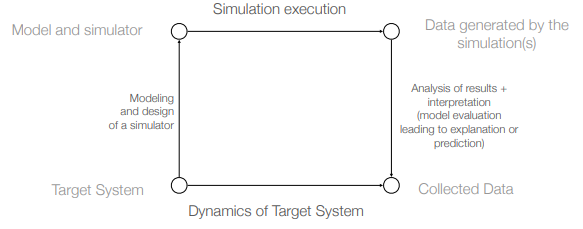
\includegraphics[scale=0.5]{./img/sim/ciclobase.png}
    \caption{Ciclo di vita della simulazione}
    \label{fig:ciclo_simulazione}
\end{figure}

Possiamo suddividere quindi il processo di simulazione nelle seguenti macro-categorie:
\begin{itemize}
    \item \textbf{Sintesi}: si azzarda una sintesi del sistema reale e si crea
          un simulatore,formalizzo i fenomeni del sistema, ciò mi permette di
          definire indicatori, metriche.
    \item \textbf{Analisi}: si analizzano i risultati ottenuti dal simulatore e
          li confronto con i dati reali per validare i simulatori.
\end{itemize}
\begin{figure}
    \centering
    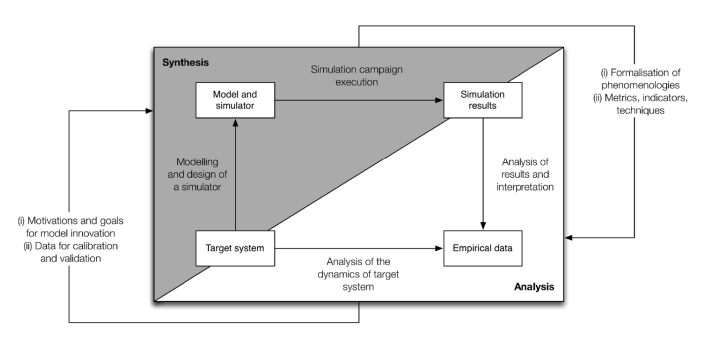
\includegraphics[scale=0.5]{./img/sim/lifecycle.png}
    \caption{Sintesi e Analisi}
    \label{fig:sintesi_analisi}
\end{figure}

Analizzando le folle di persone possiamo definire i seguenti livelli:
\begin{itemize}
    \item \textbf{Livello operazionale}: insieme di azioni che ci sono definite
          nel sistema, come ad esempio camminare, aspettare, effettuare un'attività,
          scelta della traiettoria a livello geometrico e ad ostacoli. (agente semplice)
    \item \textbf{Livello tattico} (pianifico): si discretizza il livello
          precedente spesso in un grafo, aggiungendo uno scheduling delle attività,
          scelta della strada. (base di conoscenza)
    \item \textbf{Livello strategico}
\end{itemize}
\begin{figure}
    \centering
    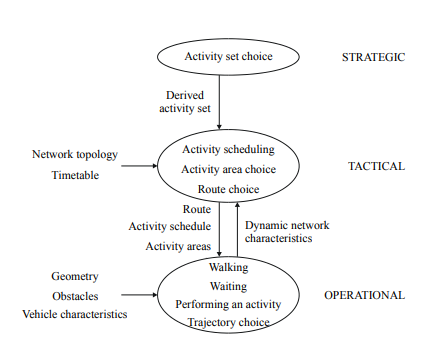
\includegraphics[scale=0.5]{./img/sim/levelsAnalysis.png}
    \caption{Livelli di analisi delle folle}
    \label{fig:livelli_folle}
\end{figure}

Possiamo modellare 2 aspetti delle folle:
\begin{itemize}
    \item \textbf{Macroscopico}: modello gli aspetti globali, spesso si specificano
          dei vincoli a livello globale (sistema di equazioni differenziali). Ha
          diversi problemi:
          \begin{itemize}
              \item Gli agenti hanno lo stesso obiettivo e comportamento.
              \item Risulta difficile da considerare gli aspetti dinamici
                    dell'ambiente perché dovremo specificare un nuovo sistema
                    differenziale che modella il secondo stato dell'ambiente e
                    abilitare i singoli sistemi in base alla tempo.
              \item Non si riescono a considerare tutti gli aspetti dinamici
                    della folla.
              \item Utile per risolvere problemi di ottimizzazione nei contesti
                    specifici.
          \end{itemize}
          Spesso sono simulazioni approssimative, si fa variale il tempo e si
          prende uno screenshot del modello a due tempi differenti. Buone
          prestazioni computazionali perché sono indipendenti dal numero
          di pedoni, però sono più limitati.
    \item \textbf{Microscopico}: si specifica il modello dei singoli agenti
          secondo la loro architettura e poi devo tener traccia degli agenti.
          Serve maggior attenzione sul sistema modellato per renderlo compatibile
          con la versione macroscopica. Con questo modello si possono sempre generare le
          stesse dinamiche aggregate della modellazione macroscopica.
          La modellazione microscopica può essere realizzata in diversi modi:
          \begin{itemize}
              \item \textbf{Particelle}: gli agenti sono particelle ma permette
                    di mantenere la componente fisica, ma si modellano i singoli
                    e non le componenti aggregate. Si specifica una velocità delle
                    particelle e si applicano delle forse su di esse anche in
                    base ai vicini. Le forze sono generate dagli obiettivi e dalle
                    altre particelle.
              \item \textbf{Automi cellulari}
          \end{itemize}
    \item \textbf{Mesoscopiche}: si hanno gli individui con delle semplificazioni
          sui loro comportamenti.
\end{itemize}

Per complicare i simulatori, perché ho parametri liberi, non posso modellare
l'eterogeneità, non posso specificare strutture particolari dell'ambiente\dots
Non esiste un approccio modellistico migliore, dipende tutto da quanto conosciamo
il fenomeno, gli obiettivi e i dati che abbiamo o misuriamo.

Simulare è difficile, passiamo dal reale alla simulazione software. Prendiamo un 
sottosistema, astraiamo il modello rimuovendo i dettagli reali, creiamo il modello 
computazionale e poi lo implementiamo. Tutte queste fasi possono essere sogette 
ad errori e inserimenti di bayes.